\clearpage
\pagestyle{fancy}
\part{Il cerchio di Mohr}
\setcounter{section}{0}
\section{La costruzione del cerchio di Mohr}
%----------------------------------------------------------------------------------------
\renewcommand{\thefigure}{5~-~1}
\begin{figure}[h]
\centering
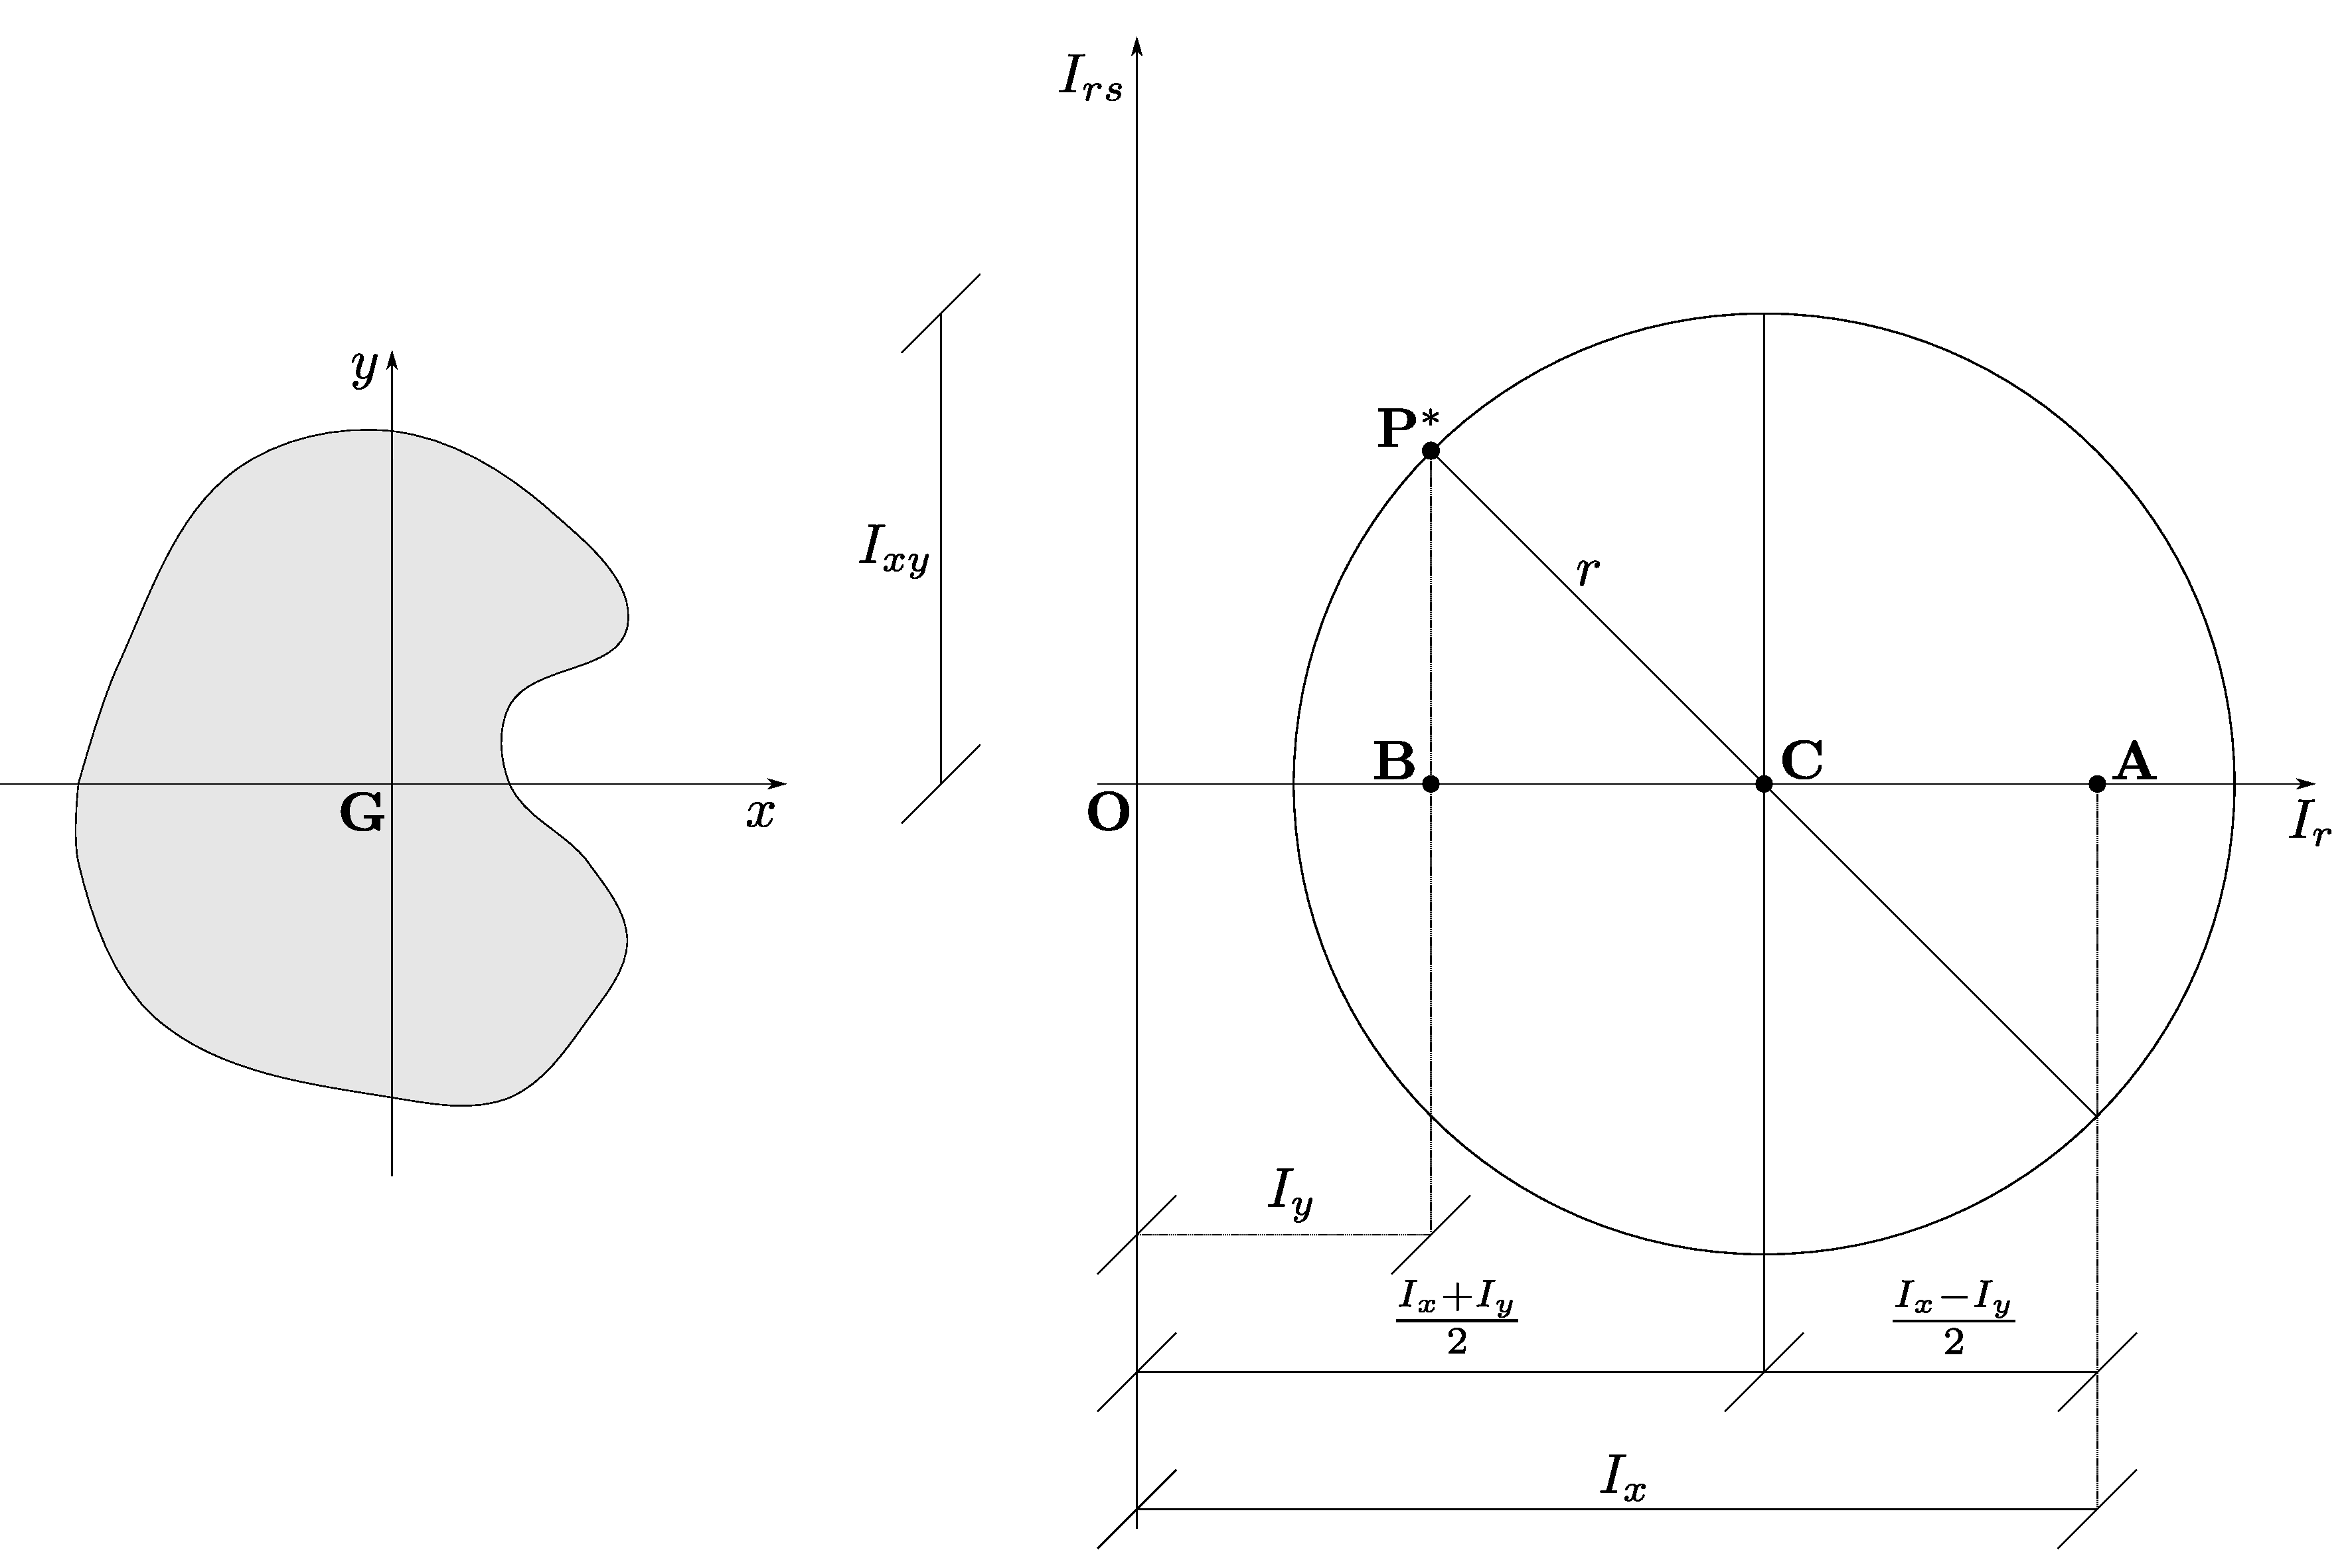
\includegraphics[width=\textwidth]{Immagini/Parte_5/Figura5_1/Figura5_1.pdf}
\caption{}
\label{figura5-1}
\end{figure}
%----------------------------------------------------------------------------------------
%--------------------------------------------------------------------------------------------------------------------------------------------------------------
\noindent Noti $I_x$, $I_y$ ed $I_{xy}$ di una data figura piana, l'origine del riferimento esendo in $\mathbf{G}$, abbiamo visto come sia possibile, grazie alla~\eqref{equazione4-2}, determinare gli assi principali $\xi$ ed $\eta$ e, grazie alle prime due delle~\eqref{equazione4-2}, calcolare $I_{\xi}$ ed $I_{\eta}$. 

\noindent Ebbene il \textsc{cerchio di Mohr} costituisce un'alternativa grafica al suddetto procedimento analitico. Noti $I_x$, $I_y$ ed $I_{xy}$ della figura piana in questione, per costruire il cerchio di Mohr si procede come segue (si faccia riferimento alla figura~\ref{figura5-1}):
%--------------------------------------------------------------------------------------------------------------------------------------------------------------
\begin{enumerate}
\item si disegnano, con origine arbitraria, le due rette $I_r$ ed $I_{rs}$ parallele e concordi ad $x$ ed $y$;
\item si assume (a piacere) una scala che traduca in $[\textup{cm}]$ i valori di $I_x$, $I_y$ ed $I_{xy}$;
\item nel riferimento $\mathbf{O}I_{r}I_{rs}$ si evidenziano i punti 
%--------------------------------------------------------------------------------------------------------------------------------------------------------------
\begin{align*}
&\mathbf{A}(I_{x},\,0) \\
&\mathbf{B}(I_{y},\,0) \\
&\mathbf{P}^{*}(I_{y},\,I_{xy}) 
\end{align*}
%--------------------------------------------------------------------------------------------------------------------------------------------------------------
\item si evidenzia il punto $\mathbf{C}$ medio del segmento $\mathbf{AB}$, la cui ascissa è ovviamente 
%--------------------------------------------------------------------------------------------------------------------------------------------------------------
\begin{equation*}
\lvert \, \mathbf{OC} \, \lvert = \frac{I_{x}+I_{y}}{2}
\end{equation*}
%--------------------------------------------------------------------------------------------------------------------------------------------------------------
\item si traccia la circonferenza di centro $\mathbf{C}$ e raggio $r=\lvert\,\mathbf{C}\mathbf{P}^{*}\lvert$: si è così costruito il cerchio di Mohr relativo alla figura piana assegnata
\end{enumerate}
%--------------------------------------------------------------------------------------------------------------------------------------------------------------
Dal disegno si evince banalmente, applicando il \textsc{teorema di Pitagora} al triangolo $\mathbf{B}\mathbf{C}\mathbf{P}^{*}$ che
%--------------------------------------------------------------------------------------------------------------------------------------------------------------
\begin{equation} \label{equazione5-1}
\boxed{r = \sqrt{\biggl(\frac{I_{x}-I_{y}}{2}\biggr)^{2}+I_{xy}^{2}}} \tag{5.1}
\end{equation}
%%--------------------------------------------------------------------------------------------------------------------------------------------------------------
\section{L'utilizzazione del cerchio di Mohr}
%----------------------------------------------------------------------------------------
\renewcommand{\thefigure}{5~-~2}
\begin{figure}[ht]
\centering
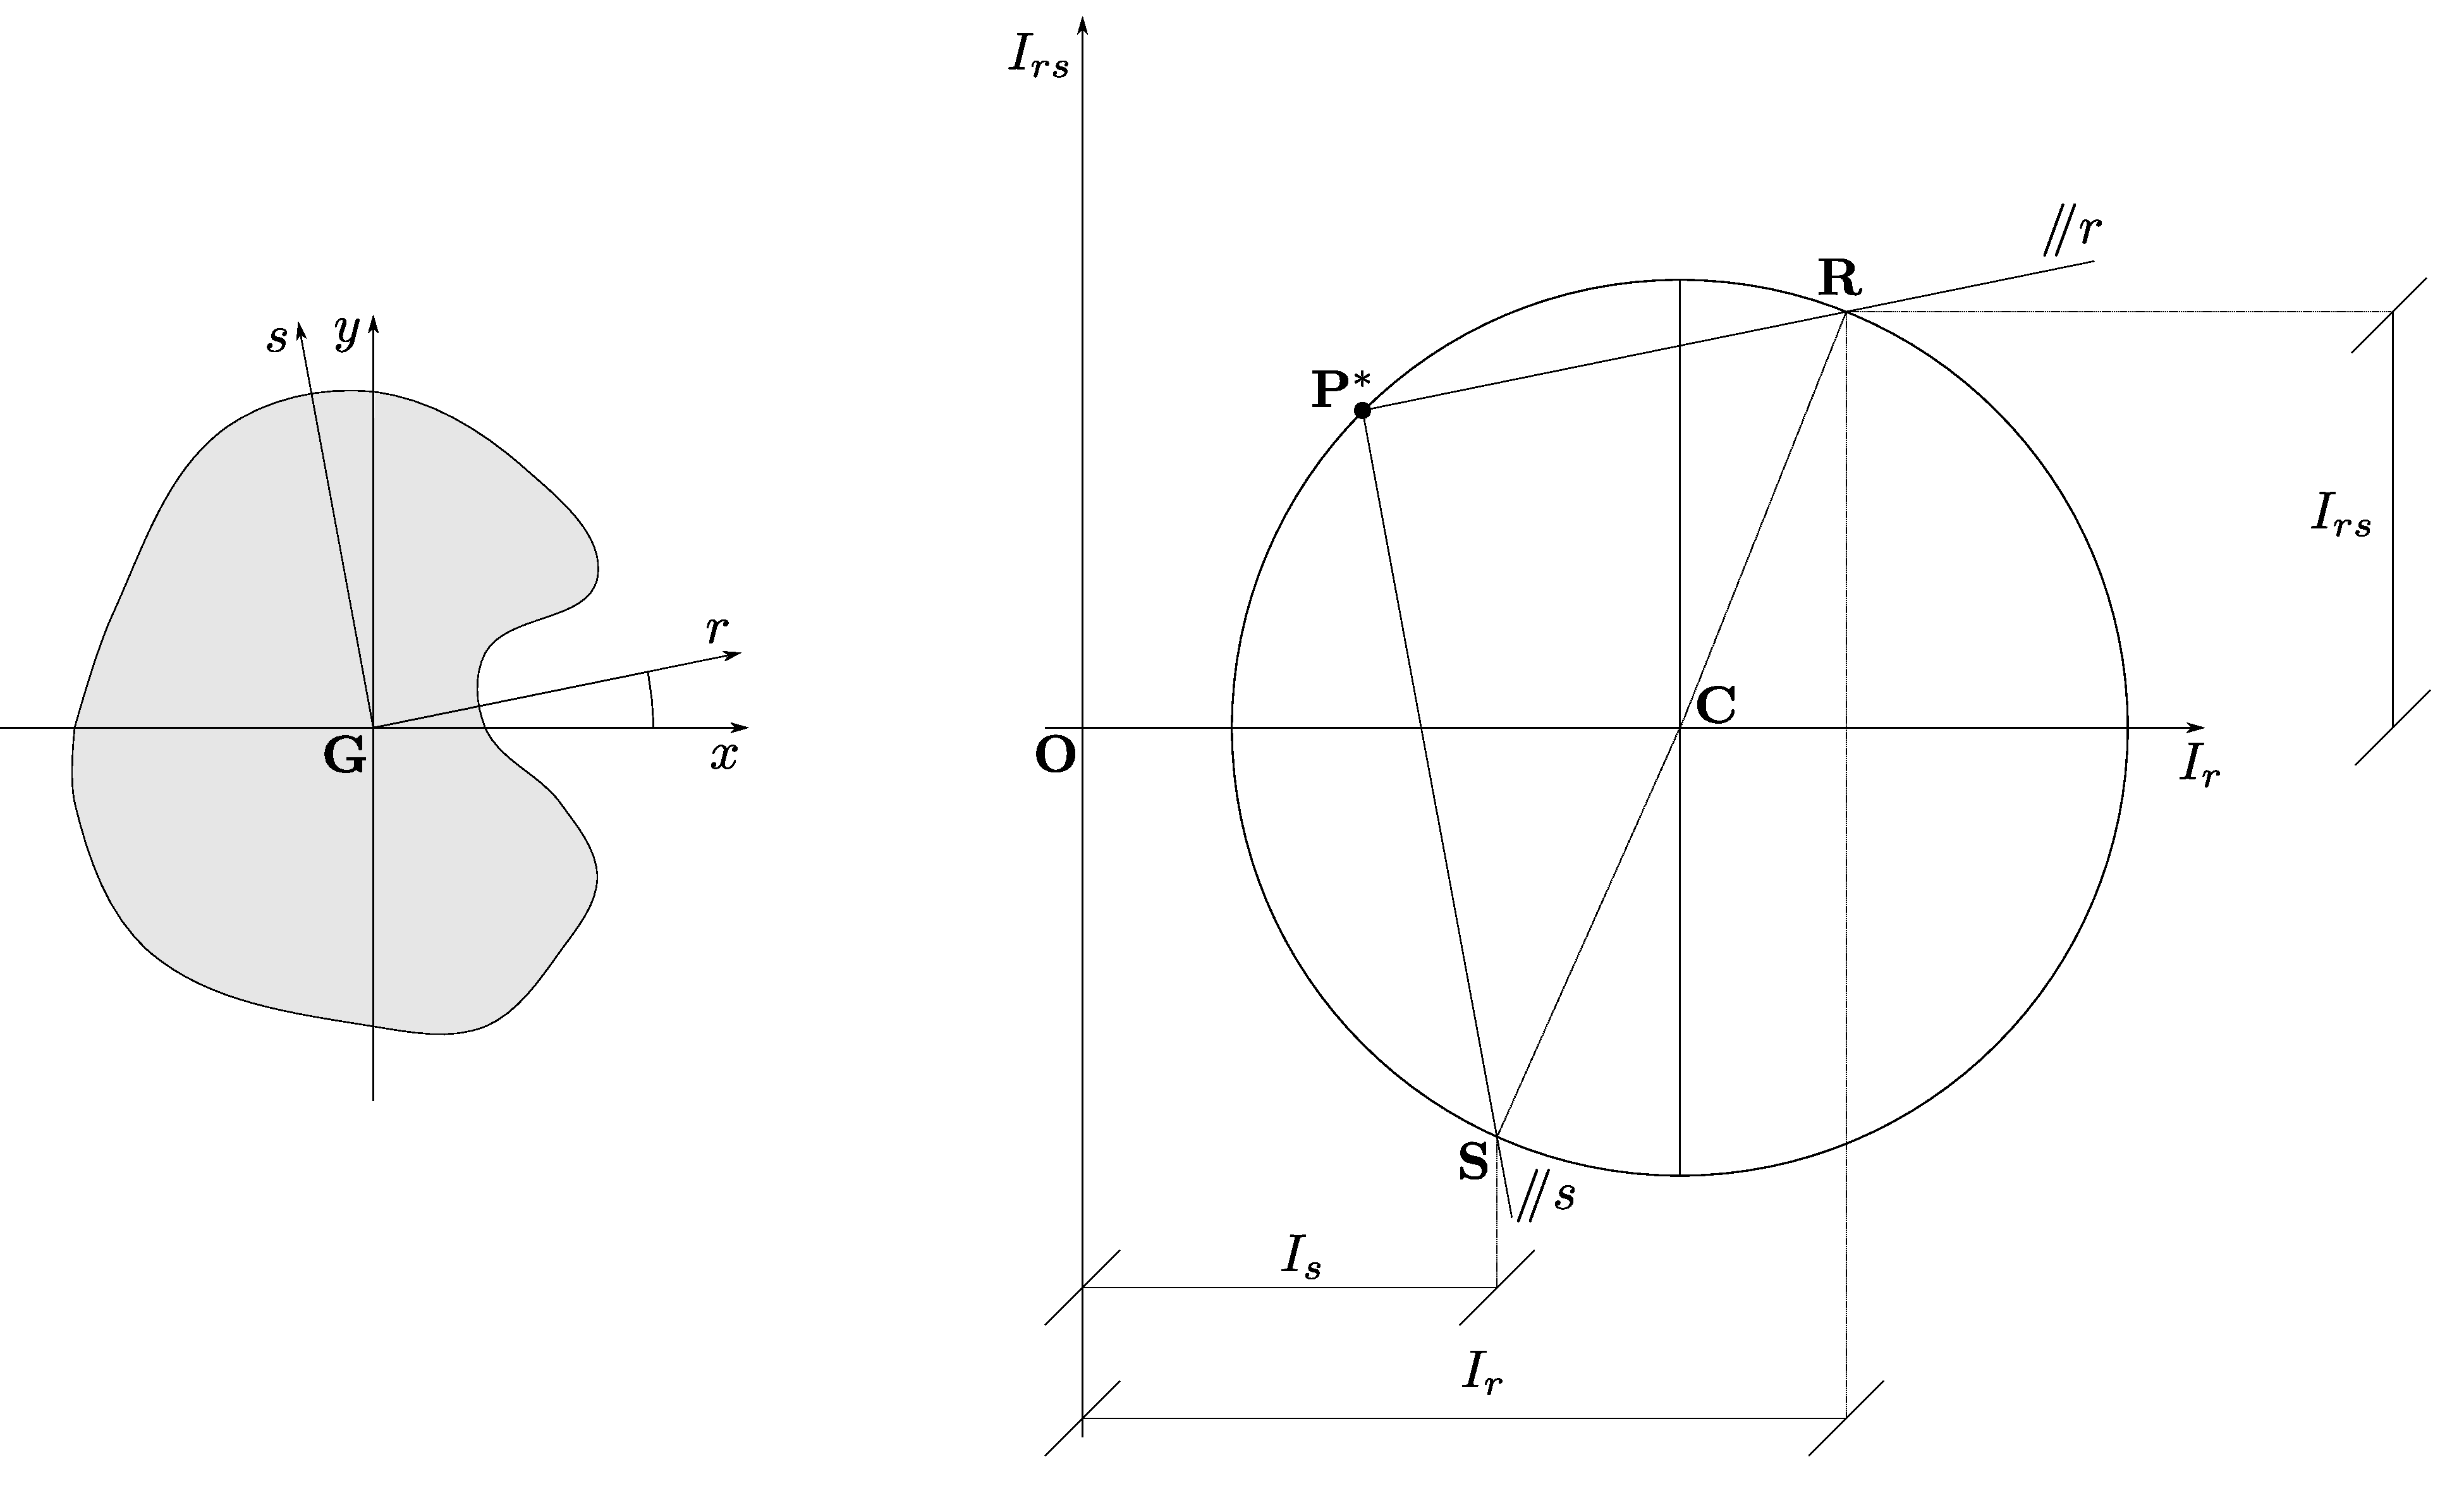
\includegraphics[width=\textwidth]{Immagini/Parte_5/Figura5_2/Figura5_2.pdf}
\caption{}
\label{figura5-2}
\end{figure}
%----------------------------------------------------------------------------------------
\noindent Con l'ausilio della figura~\ref{figura5-2}, cercheremo ora di capire come si utilizza il cerchio di Mohr. Siano $r$ ed $s$ due rette baricentriche, ortogonali, orientate in modo che la coppia $rs$ sia sovrapponibile alla coppia $xy$. 

\noindent Le formule~\eqref{equazione4-1} consentono, noti $I_x$, $I_y$ ed $I_{xy}$ di calcolare $I_r$, $I_s$ ed $I_{rs}$ identificando con $r$ l'asse $x'$ e con $s$ l'asse $y'$; ma noi, in questo paragrafo, vedremo come è possibile ottenere i valori di $I_r$, $I_s$ ed $I_{rs}$ grazie al cerchio di Mohr.
%--------------------------------------------------------------------------------------------------------------------------------------------------------------

\noindent Si tracciano per $\mathbf{P}^{*}$ le parallele ad $r$ e ad $s$; esse intersecano la circonferenza rispettivamente nei punti $\mathbf{R}$ ed $\mathbf{S}$; essendo le rette $r$ ed $s$ ortogonali, consegue che i punti $\mathbf{R}$ ed $\mathbf{S}$ sono \textsc{diametralmente opposti}. Ebbene, in forza della~\eqref{equazione4-1}, si potrebbe dimostrare che
%--------------------------------------------------------------------------------------------------------------------------------------------------------------
\begin{align*}
\textup{\textsc{Ascissa di }}\mathbf{R} &= I_r \\
\textup{\textsc{Ascissa di }}\mathbf{S} &= I_s \\
\textup{\textsc{Ordinata di }}\mathbf{R} &= I_{rs} 
\end{align*}
%--------------------------------------------------------------------------------------------------------------------------------------------------------------
%----------------------------------------------------------------------------------------
\renewcommand{\thefigure}{5~-~3}
\begin{figure}[ht]
\centering
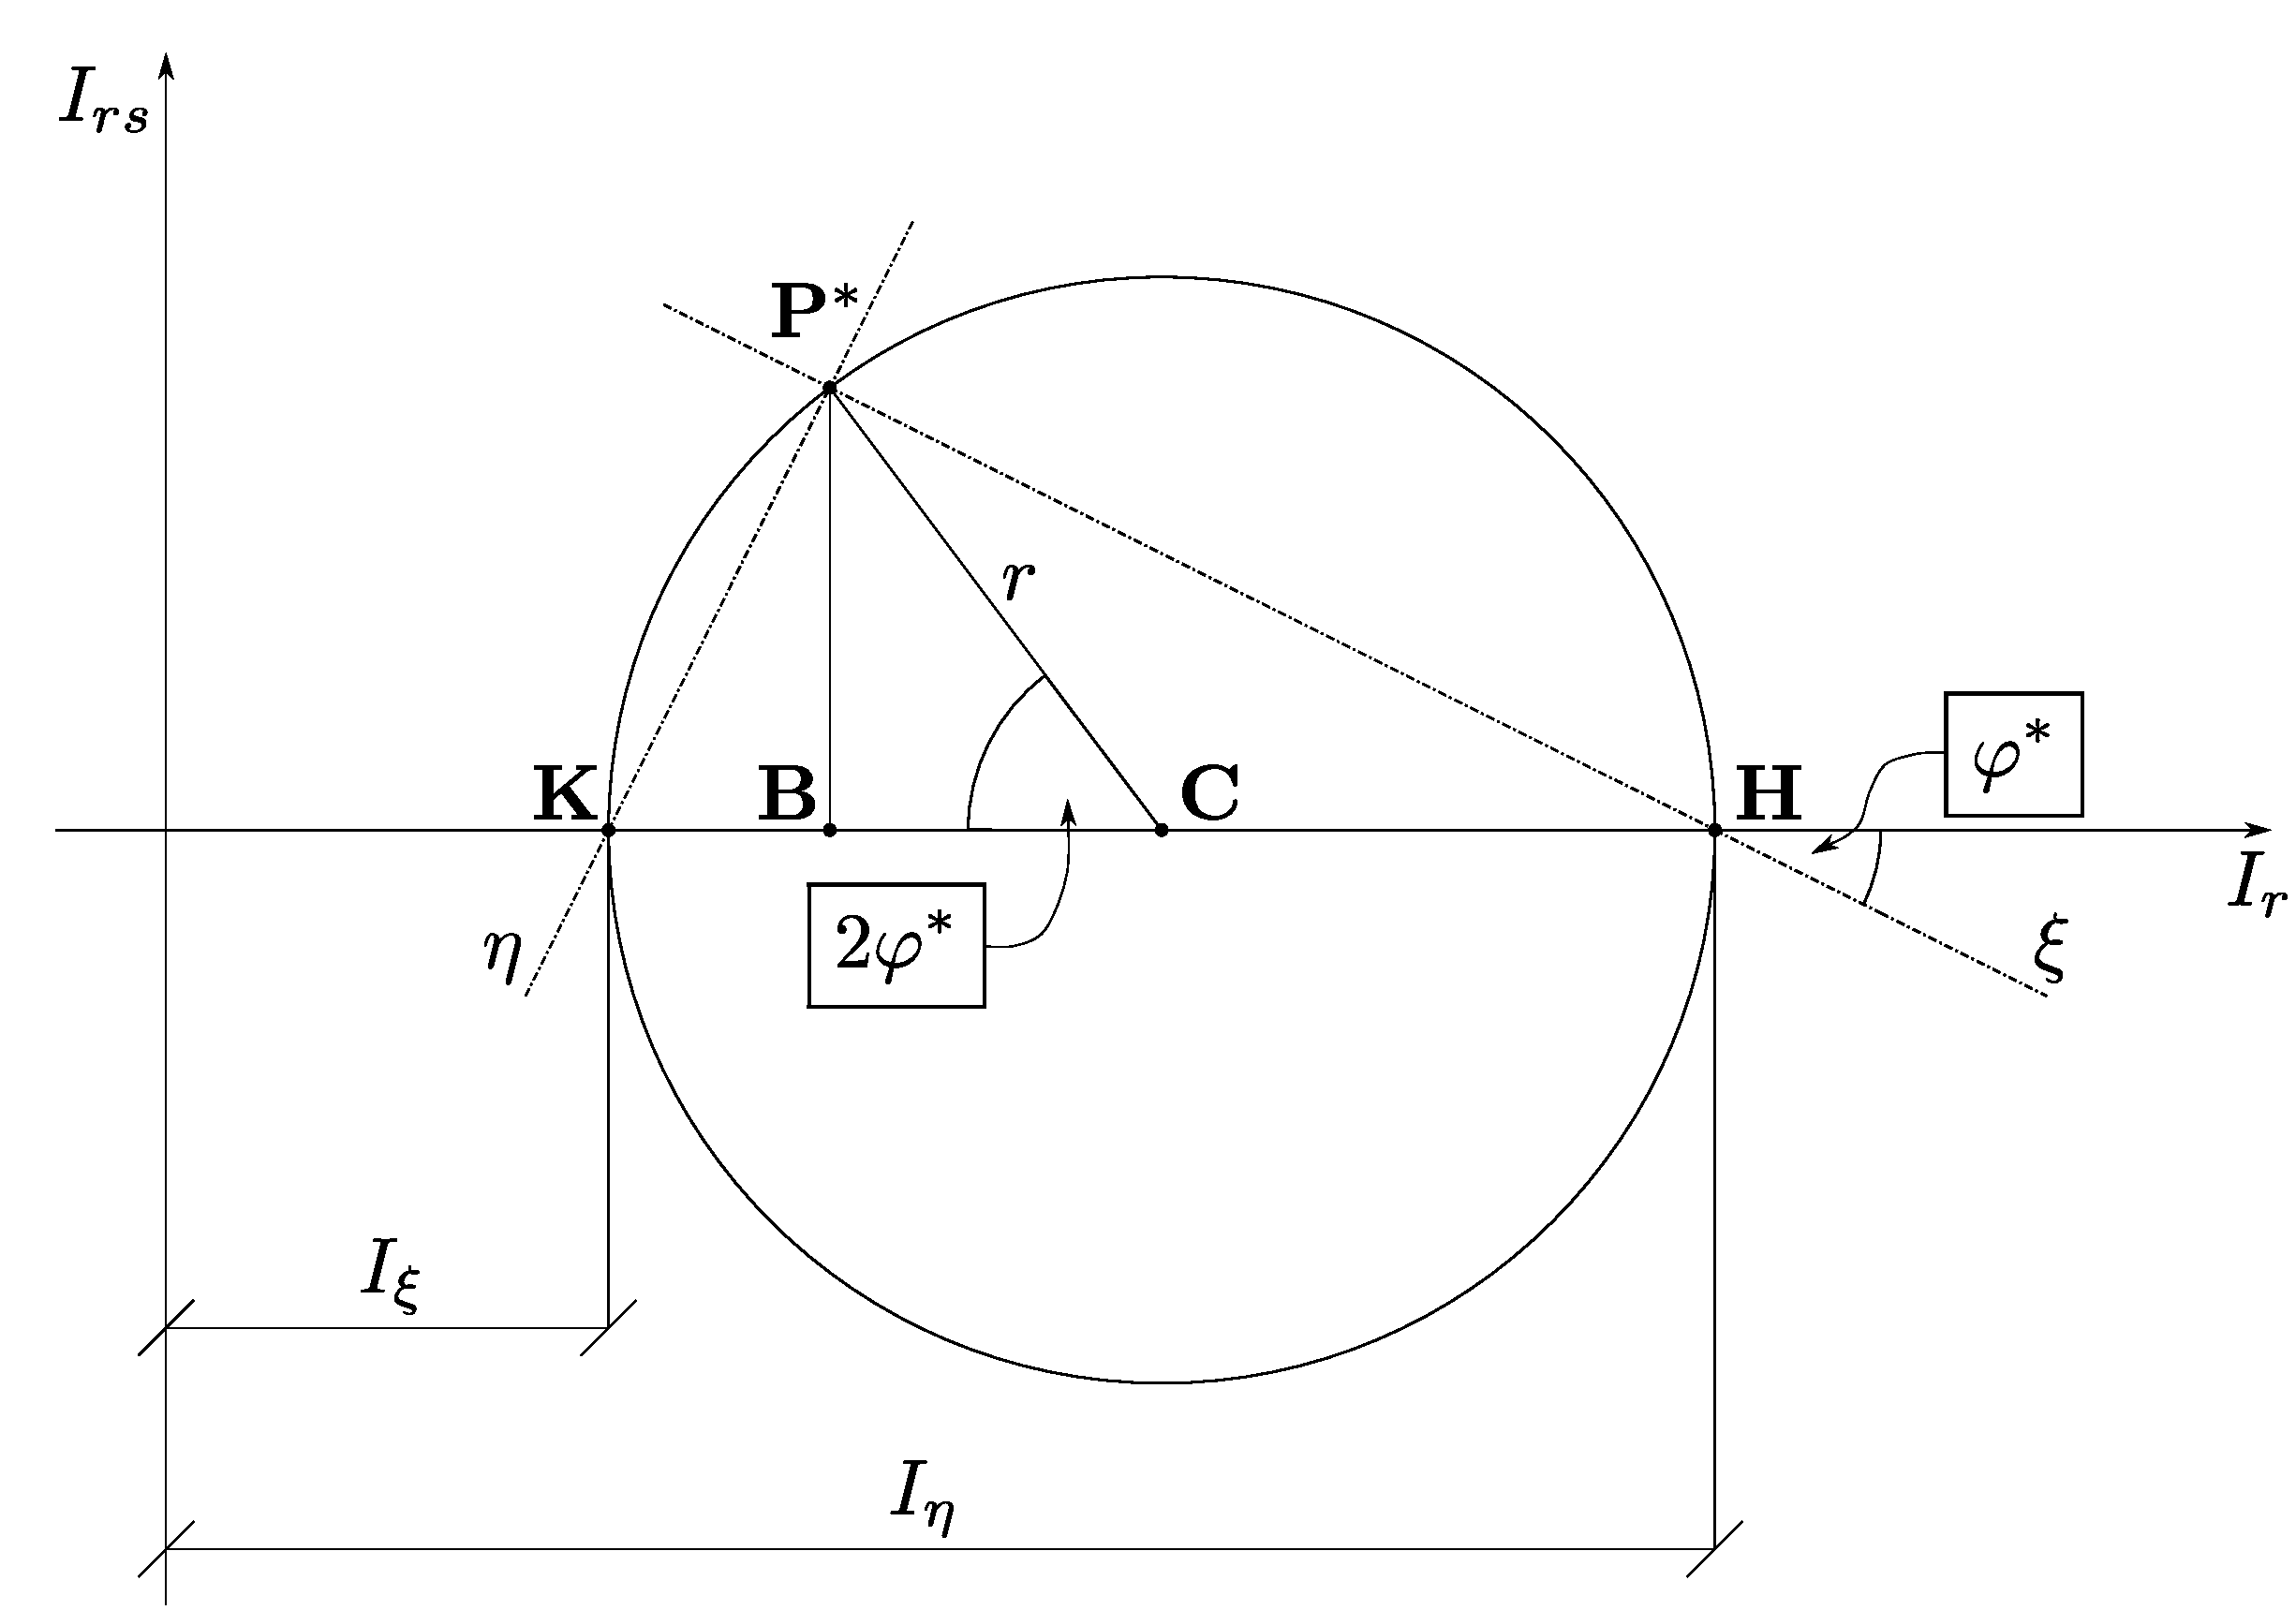
\includegraphics[width=\textwidth]{Immagini/Parte_5/Figura5_3/Figura5_3.pdf}
\caption{}
\label{figura5-3}
\end{figure}
%----------------------------------------------------------------------------------------
Facciamo ora riferimento alla figura~\ref{figura5-3}: qui sono evidenziati i punti $\mathbf{H}$ e $\mathbf{K}$, estremi del diametro orizzontale. Le rette che congiungono $\mathbf{P}^{*}$ con $\mathbf{H}$ e $\mathbf{K}$ sono evidentemente caratterizzate dai seguenti requisiti:
%--------------------------------------------------------------------------------------------------------------------------------------------------------------
\begin{enumerate}
\item sono ortogonali
\item è nullo il momento centrifugo rispetto ad esse, essendo nulle le ordinate dei punti $\mathbf{H}$ e $\mathbf{K}$
\item i momenti di inerzia rispetto ad esse sono uno \textsc{massimo} e l'altro \textsc{minimo}, tali essendo le ascisse dei punti $\mathbf{H}$ e $\mathbf{K}$
\end{enumerate}
%--------------------------------------------------------------------------------------------------------------------------------------------------------------
Si riconosce, così, che le rette in questione sono gli assi principali di inerzia.
%--------------------------------------------------------------------------------------------------------------------------------------------------------------
È bene sottolineare che l'asse $\xi$ coinciderà con quella, delle due rette $\mathbf{P}^{*}\mathbf{H}$ e $\mathbf{P}^{*}\mathbf{P}$, che forma con l'asse $I_r$ l'angolo \textsc{minore}. Il valore $\varphi^{*}=\widehat{\xi x}$ si può dedurre agevolmente dalla figura~\ref{figura5-3}. Con semplici considerazioni geometriche si trova che:
%--------------------------------------------------------------------------------------------------------------------------------------------------------------
\begin{equation*}
\tan 2\varphi^{*} = -\frac{\lvert \,\mathbf{B}\mathbf{P}^{*} \,\lvert}{\lvert \,\mathbf{B}\mathbf{C} \,\lvert}
\end{equation*}
%--------------------------------------------------------------------------------------------------------------------------------------------------------------
Il segno meno si giustifica alla luce del fatto che, in figura~\ref{figura5-3}, $\varphi^{*}$ risulta essere negativo perché orario. E poiché
%--------------------------------------------------------------------------------------------------------------------------------------------------------------
\begin{align*}
\lvert \, \mathbf{B}\mathbf{P}^{*}\,\lvert &= I_{xy} \\ 
\lvert \, \mathbf{B}\mathbf{C}\,\lvert &= \frac{I_{x}-I_{y}}{2} 
\end{align*}
%--------------------------------------------------------------------------------------------------------------------------------------------------------------
si trova
%--------------------------------------------------------------------------------------------------------------------------------------------------------------
\begin{equation*}
\tan 2\varphi^{*} = -\frac{2I_{xy}}{I_{x}-I_{y}}
\end{equation*}
%--------------------------------------------------------------------------------------------------------------------------------------------------------------
relazione che, riconosciamo, essere coincidente con la~\eqref{equazione4-2} qui ritrovata attraverso il cerchio di Mohr.
%--------------------------------------------------------------------------------------------------------------------------------------------------------------

\noindent Dalla figura~\ref{figura5-3} appare inoltre evidente che 
%--------------------------------------------------------------------------------------------------------------------------------------------------------------
\begin{align*}
I_{\xi} &= \lvert \, \mathbf{O}\mathbf{H} \, \lvert = \lvert \, \mathbf{O}\mathbf{C} \, \lvert + r \\
I_{\eta} &= \lvert \, \mathbf{O}\mathbf{K} \, \lvert = \lvert \, \mathbf{O}\mathbf{C} \, \lvert - r 
\end{align*}
%--------------------------------------------------------------------------------------------------------------------------------------------------------------
e cioè, per quanto si è visto dalla~\eqref{equazione5-1}
%--------------------------------------------------------------------------------------------------------------------------------------------------------------
\begin{equation*}
\begin{aligned}
I_{\xi} & \\
I_{\eta} &
\end{aligned}
\,\,\Biggr\}\,\, \frac{I_{x}+I_{y}}{2} \pm \sqrt{\biggl(\frac{I_{x}-I_{y}}{2}\biggr)^{2}+I_{xy}^{2}}
\end{equation*}
%--------------------------------------------------------------------------------------------------------------------------------------------------------------
La precedente formula è, forse, lo strumento più efficace per calcolare $I_{\xi}$ ed $I_{\eta}$; l'alternativa, come sappiamo, è utilizzare le prime due delle~\eqref{equazione4-1} ponendo in esse $\varphi^{*}$ in luogo di $\varphi$; tuttavia è opportuna una precisazione: in essa compare il simbolo $\pm$ dove il $+$ è riferito ad $I_{\xi}$ ed il $-$ ad $I_{\eta}$; ebbene ciò è vero se 
%--------------------------------------------------------------------------------------------------------------------------------------------------------------
\begin{equation*}
\boxed{I_{x} > I_{y}}
\end{equation*}
%--------------------------------------------------------------------------------------------------------------------------------------------------------------
Se invece $I_{x}<I_{y}$, bisognerà porre $\mp$ in essa. In definitiva 
%--------------------------------------------------------------------------------------------------------------------------------------------------------------
\begin{align}
\boxed{\textup{\textsc{se }}I_{x} > I_{y}} &\longrightarrow \boxed{\frac{I_{x}+I_{y}}{2} \pm \sqrt{\biggl(\frac{I_{x}-I_{y}}{2}\biggr)^{2}+I_{xy}^{2}}}\tag{5.2a} \label{equazione5-2a} \\
\boxed{\textup{\textsc{se }}I_{x} < I_{y}} &\longrightarrow \boxed{\frac{I_{x}+I_{y}}{2} \mp \sqrt{\biggl(\frac{I_{x}-I_{y}}{2}\biggr)^{2}+I_{xy}^{2}}} \tag{5.2b} \label{equazione5-2b}
\end{align}
%--------------------------------------------------------------------------------------------------------------------------------------------------------------
\clearpage
\section{Esercizi}
\paragraph{Esercizio 5.1}

\noindent Con riferimento al profilato dell'Esercizio 4.1, si richiede
\begin{enumerate}
\item di costruire il cerchio di Mohr;
\item di calcolare $I_{\xi}$ ed $I_{\eta}$ utilizzando le relazioni~\eqref{equazione5-2a} e~\eqref{equazione5-2b};
\item di individuare la coppia di rette, ortogonali e baricentriche, rispetto a cui è massimo il momento centrifugo e trovarne il valore;
\item di trovare il valore dei momenti di inerzia di cui in 3;
\item di determinare sia graficamente che analiticamente, i valori di $I_r$, $I_s$ ed $I_{rs}$, essendo $r$ la retta che forma con $x$ l'angolo di $45^{\circ}$.
\end{enumerate}
%--------------------------------------------------------------------------------------------------------------------------------------------------------------

\noindent \subparagraph{Quesito 1}  Sappiamo già che (si riveda l'Esercizio 4.1)
%--------------------------------------------------------------------------------------------------------------------------------------------------------------
\begin{align*}
I_x &= 16155\,\textup{cm}^{4} \\
I_y &= 7675\,\textup{cm}^{4} \\
I_{xy} &= -7966\,\textup{cm}^{4}
\end{align*}
%--------------------------------------------------------------------------------------------------------------------------------------------------------------
I connotati del cerchio di Mohr del profilato in questione, sono, dunque:
%--------------------------------------------------------------------------------------------------------------------------------------------------------------
\begin{align*}
\lvert \, \mathbf{O}\mathbf{C}\,\lvert &= \frac{I_{x}+I_{y}}{2} = 11915\,\textup{cm}^{4} \\
r &= \sqrt{\biggl(\frac{I_{x}-I_{y}}{2}\biggr)^{2}+I_{xy}^{2}} = 9024\,\textup{cm}^{4}
\end{align*}
%--------------------------------------------------------------------------------------------------------------------------------------------------------------
Alla luce di questi connotati, andiamo a stabilire la \textsc{scala} con cui trasformeremo in $\textup{cm}$ i momenti del secondo ordine. Se vogliamo che il cerchio entri in un foglio come questo, con formato \textsc{a}$4$, dobbiamo far sì che il suo raggio sia nettamente minore di $10\,\textup{cm}$. Assumendo la \textsc{scala momenti del secondo ordine} pari a
%--------------------------------------------------------------------------------------------------------------------------------------------------------------
\begin{equation*}
1\,\textup{cm} = 1500\,\textup{cm}^{4}
\end{equation*}
%--------------------------------------------------------------------------------------------------------------------------------------------------------------
avremo un raggio
%--------------------------------------------------------------------------------------------------------------------------------------------------------------
\begin{equation*}
r = \frac{9024}{1500} \approx 6\,\textup{cm}
\end{equation*}
%--------------------------------------------------------------------------------------------------------------------------------------------------------------
Le coordinate sul cerchio di Mohr del polo $\mathbf{P}^{*}$ sono, conseguentemente 
%--------------------------------------------------------------------------------------------------------------------------------------------------------------
\begin{equation*}
\mathbf{P}^{*}(I_y,\,I_{xy}) \rightarrow \mathbf{P}^{*}\biggl(\frac{7675}{1500},\,-\frac{7966}{1500}\biggr) \rightarrow \mathbf{P}^{*}(5.12\,\textup{cm},\,-5.31\,\textup{cm})
\end{equation*}
%--------------------------------------------------------------------------------------------------------------------------------------------------------------
Il lettore è invitato a controllare la coincidenza di questi risultati con quelli trovati alla fine dell'Esercizio 4.1.
%--------------------------------------------------------------------------------------------------------------------------------------------------------------
%----------------------------------------------------------------------------------------
\renewcommand{\thefigure}{5.1~-~1}
\begin{figure}[ht]
\centering
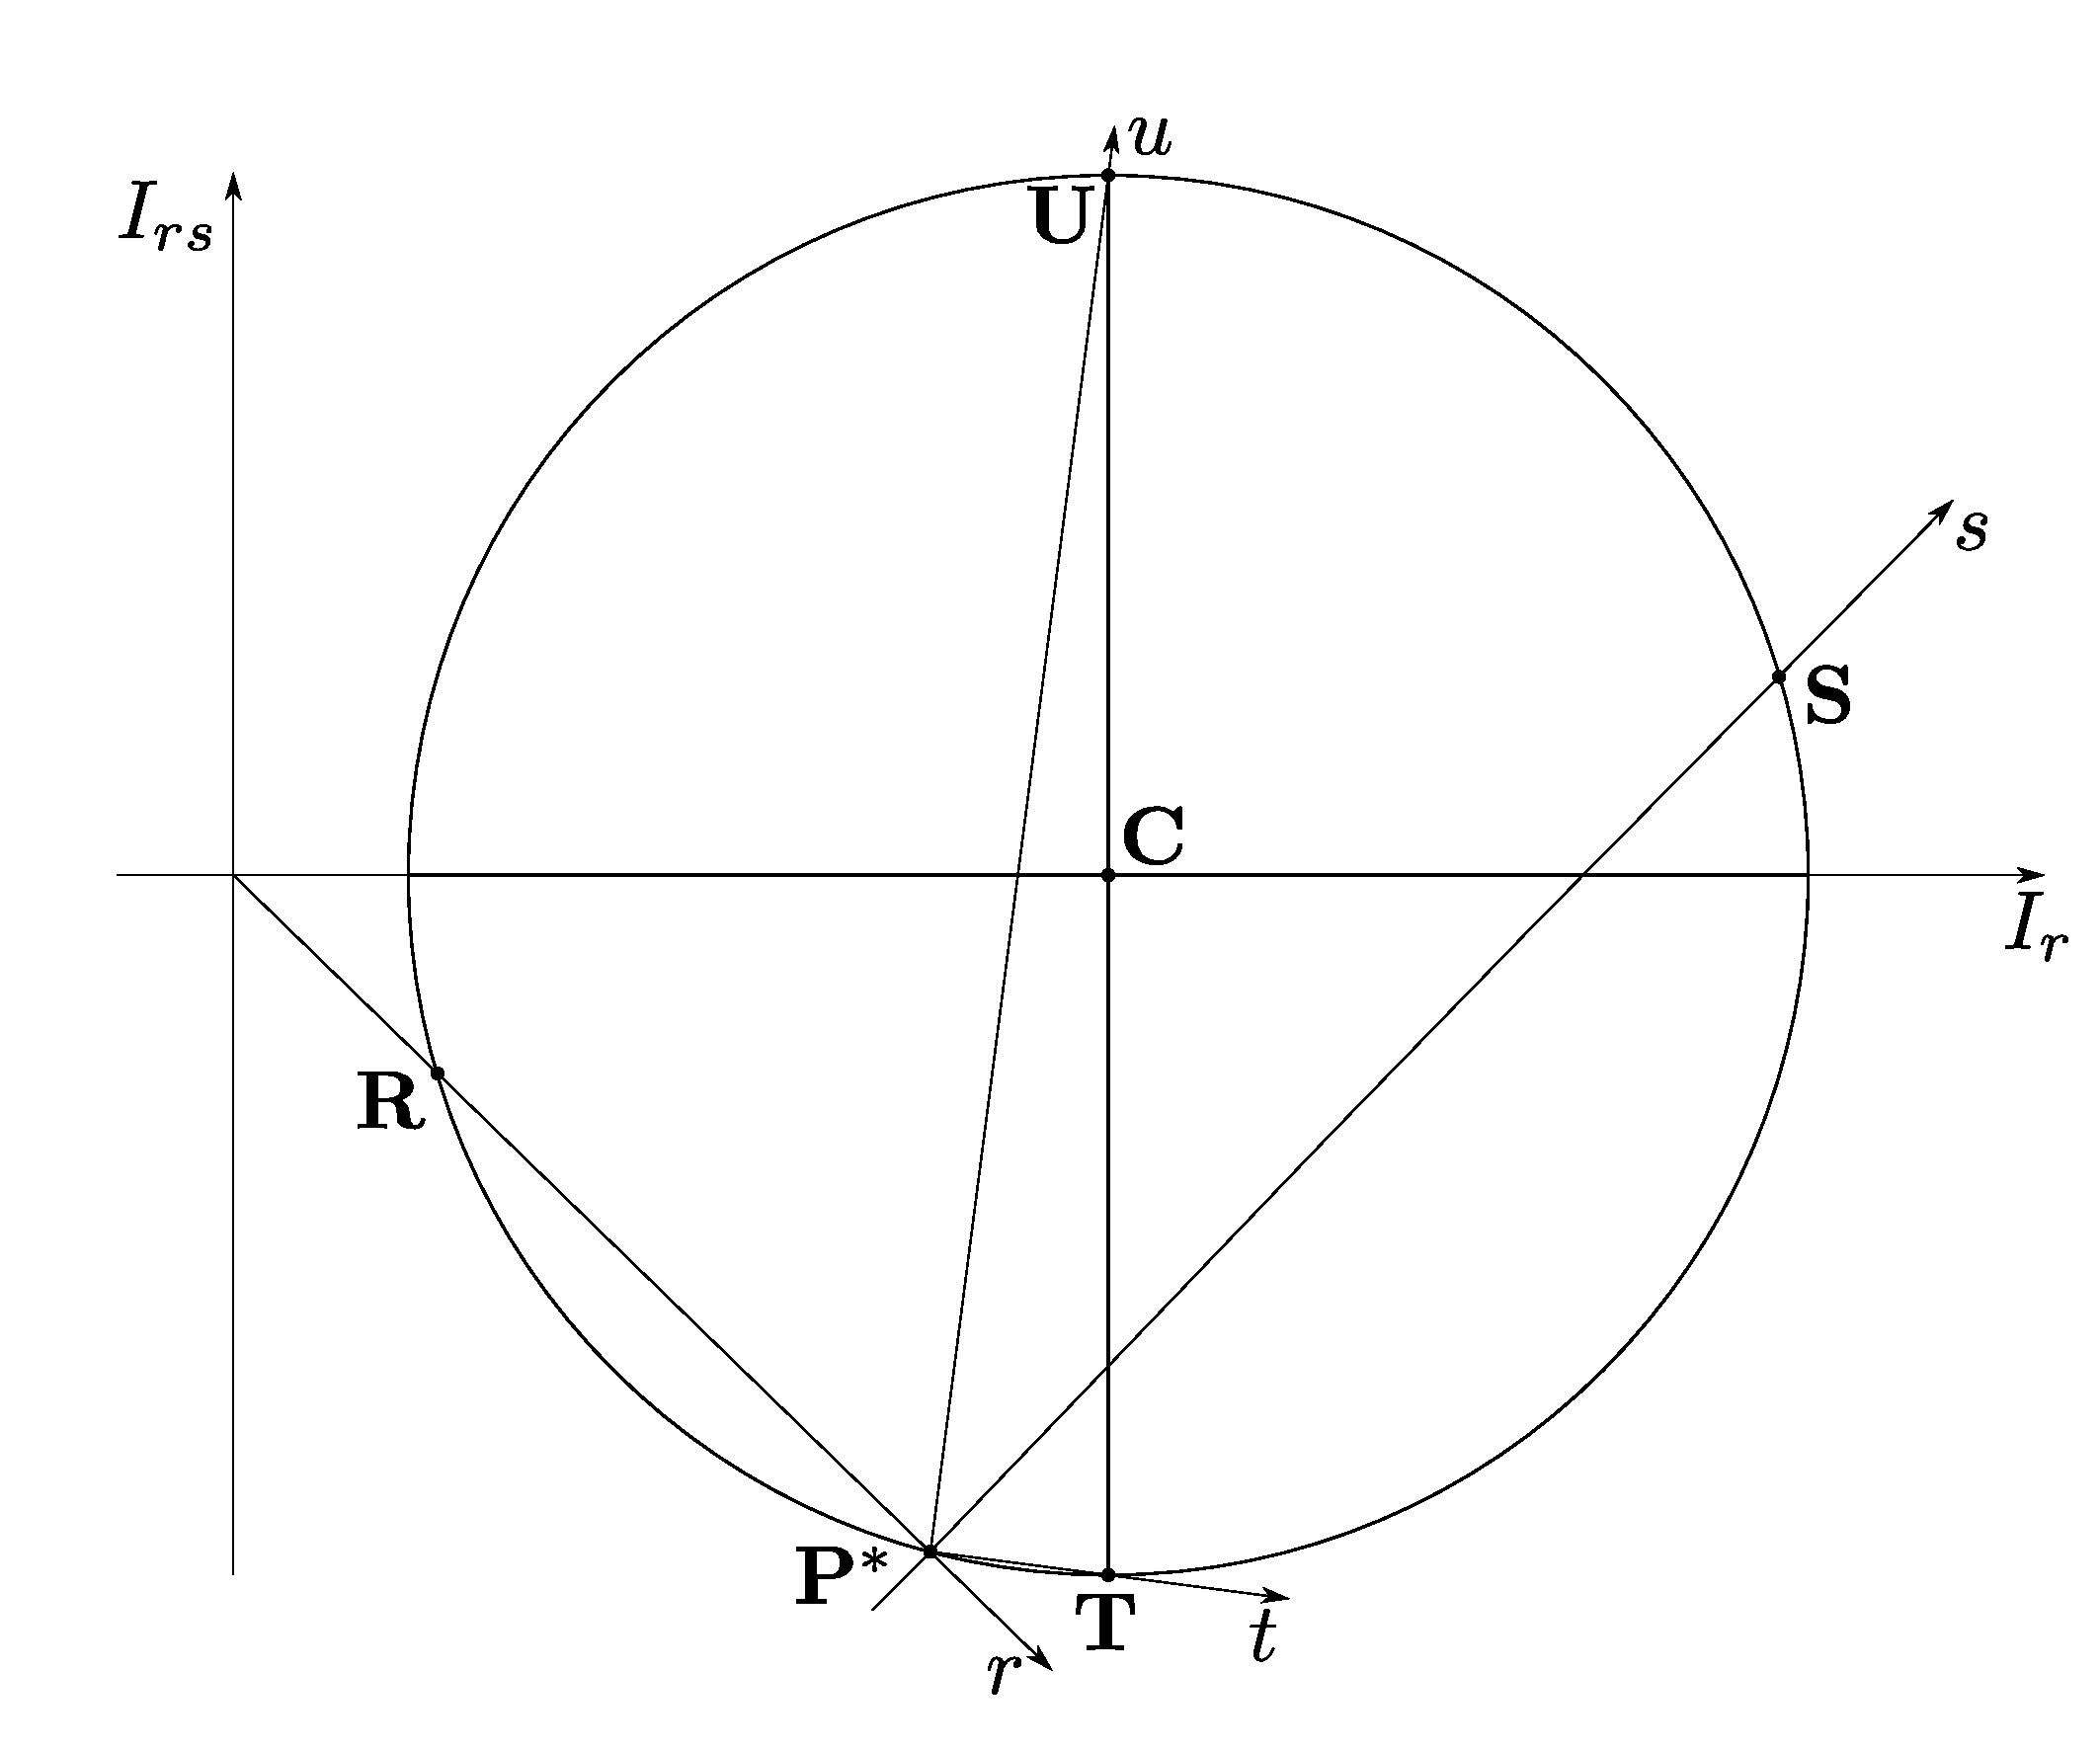
\includegraphics[width=\textwidth]{Immagini/Parte_5/Esercizio5_1/Esercizio5_1_1.pdf}
\caption{}
\label{Esercizio5-1-1}
\end{figure}
%----------------------------------------------------------------------------------------
\noindent \subparagraph{Quesito 3} La coppia di rette rispetto alle quali è massimo il momento centrifugo è, ovviamente, quella che si ottiene congiungendo il polo $\mathbf{P}^{*}$ con i punti $\mathbf{T}$ ed $\mathbf{U}$ estremi del diametro verticale. Orientate le rette $\mathbf{P}^{*}\mathbf{T}=t$ e $\mathbf{P}^{*}\mathbf{U}=u$ come in figura, chiaramente risulta:
%--------------------------------------------------------------------------------------------------------------------------------------------------------------
\begin{equation*}
I_{tu} = \textup{\textsc{ordinata di }}\mathbf{T} = -r = -9024\,\textup{cm}^{4}
\end{equation*}
%--------------------------------------------------------------------------------------------------------------------------------------------------------------
\noindent \subparagraph{Quesito 4} Chiaramente 
%--------------------------------------------------------------------------------------------------------------------------------------------------------------
\begin{equation*}
I_t = I_u = \lvert\, \mathbf{O}\mathbf{C}\,\lvert = 11915\,\textup{cm}^{4}
\end{equation*}
%--------------------------------------------------------------------------------------------------------------------------------------------------------------
\noindent \subparagraph{Quesito 5} La retta $r$ e la sua normale $s$ si sono disegnate sempre sul cerchio in figura; esse si sono orientate così che la coppia $rs$ sia sovrapponibile alla coppia $xy$; abbiamo indicato, naturalmente, con $\mathbf{R}$ ed $\mathbf{S}$ le rispettive intersezioni di $r$ ed $s$ con la circonferenza. E, dunque, dal disegno si rileva
%--------------------------------------------------------------------------------------------------------------------------------------------------------------
\begin{align*}
I_r &= \textup{\textsc{ascissa di }} \mathbf{R} \cong 2.60\,\textup{cm} \longrightarrow 3900\,\textup{cm}^{4} \\
I_s &= \textup{\textsc{ascissa di }} \mathbf{S} \cong 13.25\,\textup{cm} \longrightarrow 19875\,\textup{cm}^{4} \\
I_{rs} &= \textup{\textsc{ordinata di }}\mathbf{R} \cong -2.80\,\textup{cm} \longrightarrow -4200\,\textup{cm}^{4}
\end{align*}
%--------------------------------------------------------------------------------------------------------------------------------------------------------------
Applicando le~\eqref{equazione4-1}, ponendo in esse $\varphi^{*}=45^{\circ}$, si trova che
%--------------------------------------------------------------------------------------------------------------------------------------------------------------
\begin{align*}
I_r &= 3949\,\textup{cm}^{4} \\
I_s &= 19881\,\textup{cm}^{4} \\
I_{rs} &= 4240\,\textup{cm}^{4} 
\end{align*}
%--------------------------------------------------------------------------------------------------------------------------------------------------------------
Naturalmente i valori \textsc{esatti} sono questi ultimi; lo scarto, peraltro molto modesto, è dovuto all'inevitabile errore nella misura delle distanze sul disegno in scala.
%--------------------------------------------------------------------------------------------------------------------------------------------------------------